\section{Test af Matrix Multiplatikon}
I denne det vil resultaterne af testende på en computer med udstyret blive vist:
\begin{itemize}
\item styresystem: Windows 10 Pro N
\item Processor: intel core i5-4690K
\item Hukommelse (RAM): 12 GB
\item Skærmkort: NVIDIA GeForce GTX 960
\end{itemize}

\subsection{Resultater fra Programmerne} \label{result_GPU_Funcalc}
resultater vil blive delt op efter hvad tiden er blevet målt igennem, C\# og C++. Dette er gjort fordi at C\# har muligheden for at måle i tid, kan man ikke rigtig måle i tid i C++. I C++ kan man bruge biblioteket \textit{time.h}, problemet med dette biblioteket er, at det måler i \textit{clock ticks}, der er en tidsenhed af en konstant, men systemspecifikke længde. Der findes en macro \textit{CLOCKS\_ PER\_ SEC}, som burde gøre arbejde, men med mine test kan kan jeg ikke se hvordan det passer sammen med hvad jeg får med mine C\# målinger.

På tabel \ref{fig:samletCS} kan målingerne fra C\# ses og på tabel \ref{fig:samletC++} kan målingerne fra C++ ses. C++ AMP med to dimensioner array skete der en stack overflow da array blev på størrelse 300 x 300 eller over.

% ------------------------------------------------------------------------------------------------------------- samlet C#
\begin{figure}[p]
    \centering
   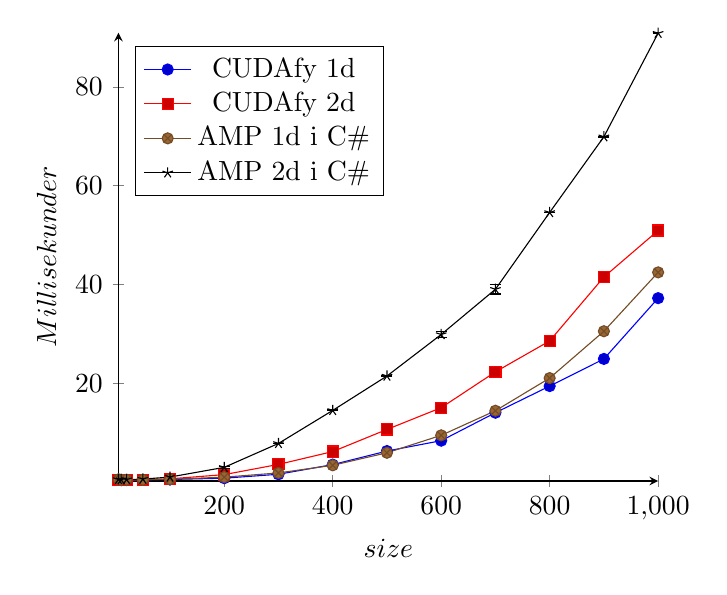
\begin{tikzpicture} 
\begin{axis}
[
    axis lines = left,
    xlabel = $size$,
    ylabel = $Millisekunder$,
    legend pos=north west,
]

 \addplot+[error bars/.cd,y dir=both,y explicit]
	coordinates 
    	{ 	
		(5,0.533) +- (0,0.147)
		(10,0.478) +- (0,0.019)
		(20,0.487) +- (0, 0.010)
		(50,0.543) +- (0,0.012)
		(100,0.607) +- (0,0.012)
		(200,0.87) +- (0,0.013)
		(300, 1.661) +- (0,0.041)
		(400,3.617) +- (0,0.047)
		(500,6.359) +- (0,0.107)
		(600,8.456) +- (0,0.096)
		(700,14.109) +- (0,0.050)
		(800,19.492) +- (0,0.035)
		(900,24.987) +- (0, 0.036)
		(1000,37.275) +- (0,0.029)
 }; \addlegendentry{CUDAfy 1d}
 \addplot+[error bars/.cd,y dir=both,y explicit]
	coordinates 
    	{ 	
		(5,0.499) +- (0,0.033)
		(10,0.492) +- (0,0.010)
		(20,0.499) +- (0, 0.005)
		(50,0.56) +- (0,0.014)
		(100,0.74) +- (0,0.014)
		(200,1.594) +- (0,0.013)
		(300,3.658) +- (0,0.116)
		(400,6.251) +- (0,0.213)
		(500,10.728) +- (0,0.062)
		(600,15.122) +- (0,0.049)
		(700,22.367) +- (0,0.051)
		(800,28.626) +- (0,0.039)
		(900,41.546) +- (0, 0.025)
		(1000,50.958) +- (0,0.011)
 }; \addlegendentry{CUDAfy 2d}
 
\addplot+[error bars/.cd,y dir=both,y explicit]
	coordinates 
    	{ 	
		(5,0.637) +- (0,0.342)
		(10,0.556) +- (0,0.022)
		(20,0.56) +- (0, 0.0205)
		(50,0.552) +- (0,0.011)
		(100,0.656) +- (0,0.026)
		(200,1.076) +- (0,0.032)
		(300, 1.931) +- (0,0.046)
		(400,3.478) +- (0,0.017)
		(500,6.009) +- (0,0.018)
		(600,9.534) +- (0,0.021)
		(700,14.509) +- (0,0.023)
		(800,21.107) +- (0,0.014)
		(900,30.587) +- (0, 0.020)
		(1000,42.488) +- (0,0.039)
 };  \addlegendentry{ AMP 1d i C\#}
 
 \addplot+[error bars/.cd,y dir=both,y explicit]
	coordinates 
    	{ 	
		(5,0.611) +- (0,0.180)
		(10,0.562) +- (0,0.014)
		(20,0.581) +- (0, 0.012)
		(50,0.685) +- (0,0.007)
		(100,1.099) +- (0,0.008)
		(200,3.061) +- (0,0.232)
		(300, 7.895) +- (0,0.027)
		(400,14.574) +- (0,0.080)
		(500,21.529) +- (0,0.182)
		(600,29.924) +- (0,0.685)
		(700,39.074) +- (0,0.964)
		(800,54.605) +- (0,0.070)
		(900,69.917) +- (0, 0.117)
		(1000,90.851) +- (0,0.098)
 }; \addlegendentry{ AMP 2d i C\#}
\end{axis} \end{tikzpicture}    
    \caption{ alle målinger der er lavet i C\#}
    \label{fig:samletCS}
\end{figure}

% ------------------------------------------------------------------------------------------------------------- samlet C++
\begin{figure}[p]
    \centering
   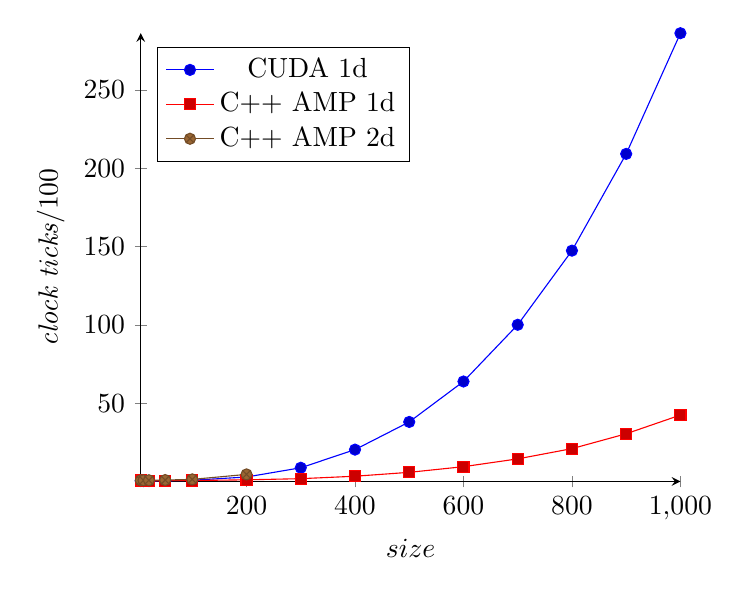
\begin{tikzpicture} 
\begin{axis}
[
    axis lines = left,
    xlabel = $size$,
    ylabel = $\textit{clock ticks}/100$,
    legend pos=north west,
]
\addplot+[error bars/.cd,y dir=both,y explicit]
	coordinates 
    	{ 	
		(5,0.542) +- (0,0.242)
		(10,0.477) +- (0,0.014)
		(20,0.498) +- (0, 0.007)
		(50,0.609) +- (0,0.008)
		(100,0.984) +- (0,0.021)
		(200,3.063) +- (0,0.035)
		(300, 8.957) +- (0,0.114)
		(400,20.526) +- (0,0.106)
		(500,38.194) +- (0,0.027)
		(600,63.997) +- (0,0.027)
		(700,100.162) +- (0,0.020)
		(800,147.458) +- (0,0.135)
		(900,209.182) +- (0, 0.025)
		(1000,286.169) +- (0,0.046)
 }; \addlegendentry{ CUDA 1d}
 
 \addplot+[error bars/.cd,y dir=both,y explicit]
	coordinates 
    	{ 	
		(5,0.826) +- (0,0.373)
		(10,0.7) +- (0,0.020)
		(20,0.694) +- (0, 0.013)
		(50,0.714) +- (0,0.034)
		(100,0.819) +- (0,0.017)
		(200,1.266) +- (0,0.021)
		(300, 1.999) +- (0,0.07)
		(400,3.56) +- (0,0.038)
		(500,6.042) +- (0,0.039)
		(600,9.649) +- (0,0.016)
		(700,14.629) +- (0,0.017)
		(800,21.16) +- (0,0.012)
		(900,30.643) +- (0, 0.027)
		(1000,42.58) +- (0,0.044)
 }; \addlegendentry{ C++ AMP 1d}
 
 \addplot+[error bars/.cd,y dir=both,y explicit]
	coordinates 
    	{ 	
		(5,0.945) +- (0,0.677)
		(10,0.948) +- (0,0.637)
		(20,0.995) +- (0, 0.769)
		(50,1.122) +- (0,0.798)
		(100,1.550) +- (0,0.771)
		(200,4.725) +- (0,0.588)
 }; \addlegendentry{ C++ AMP 2d}

\end{axis} \end{tikzpicture}    
    \caption{samlet C++}
    \label{fig:samletC++}
\end{figure}

\subsection{resultat af testen}
Ud fra testen virker det som om at CUDAfy er et godt valg til at kode i, når det skal gøres i C\# . Derfor vil GPU funktion der laves i dette projekt bruge CUDAfy til at lave GPU delen med.




